% main.tex — "The Invisible Window" IEEE Conference Paper
% Complete LaTeX conversion from docs/invisible-window-paper.md

\documentclass[conference]{IEEEtran}
\usepackage[utf8]{inputenc}
\usepackage[T1]{fontenc}
\usepackage{graphicx}
\usepackage{xcolor}
\usepackage{listings}
\usepackage{tikz}
\usepackage{hyperref}
\usepackage{amsmath,amssymb}
\usepackage{cite}
\usepackage{booktabs}
\usepackage{url}
\usetikzlibrary{shapes,arrows.meta,positioning,fit,backgrounds,calc}

% Global listings configuration
\lstset{
  basicstyle=\ttfamily\footnotesize,
  breaklines=true,
  frame=single,
  numbers=left,
  numberstyle=\tiny\color{gray},
  keywordstyle=\color{blue},
  commentstyle=\color{green!50!black},
  stringstyle=\color{red},
  columns=fullflexible
}

\begin{document}

\title{The Invisible Window: Exploiting OS-Level Display Affinity to Bypass WebRTC Proctoring Systems}

\author{\IEEEauthorblockN{Mohammad Raouf Abedini}
\IEEEauthorblockA{Department of Computing\\
Macquarie University\\
Sydney, Australia\\
mohammadraouf.abedini@students.mq.edu.au\\
https://raoufabedini.dev}
\thanks{Research conducted using Claude Code powered by Claude Opus 4.6. PoC implementations empirically validated on Windows 10 Build 19045 and macOS 26.3.1.}}

\maketitle

\begin{abstract}
Remote proctoring systems are the primary technical defence against academic misconduct in online education. These systems rely on the WebRTC \texttt{getDisplayMedia()} API to monitor test-takers' screens, operating on the implicit assumption that the captured frame faithfully represents the physical display. We demonstrate that this assumption is systematically violated by a new class of AI-powered cheating tools---including commercially available products such as Interview Coder and Cluely---that embed large language models (GPT-4, Claude) inside operating system windows rendered invisible to all screen capture mechanisms. These tools exploit documented OS-level display affinity APIs (\texttt{SetWindowDisplayAffinity} on Windows, \texttt{NSWindow.SharingType.none} on macOS) to create real-time AI assistants that are fully visible to the test-taker but produce zero pixels in proctoring capture output. Our proof-of-concept demonstrates 100\% evasion across all tested platforms---including macOS~26, where the attack was previously assumed mitigated---with zero visual artefacts and no detectable behavioural anomalies. We find that an estimated 35\% of candidates in technical assessments already show signs of AI-assisted cheating via such tools, yet no formal security analysis of this attack class exists in the academic literature. We propose countermeasures including display integrity attestation and API-level monitoring, assess their limitations, and argue that the structural vulnerability of capture-based proctoring demands a fundamental rethinking of assessment design in the age of accessible AI. This work follows coordinated vulnerability disclosure principles and is positioned at the intersection of AI security, AI-enabled misuse, and the societal impacts of generative AI on educational institutions.
\end{abstract}

\begin{IEEEkeywords}
AI-assisted cheating, display affinity, screen capture evasion, WebRTC proctoring, generative AI misuse, academic integrity, AI safety, responsible disclosure
\end{IEEEkeywords}

%% ===================================================================
%% SECTION I: INTRODUCTION
%% ===================================================================
\section{Introduction}

The global shift to online education, dramatically accelerated by the COVID-19 pandemic, has driven widespread adoption of remote proctoring technologies to safeguard academic integrity~\cite{lee2022online,noordegraaf2023ethical,khalil2022nexus}. Commercial systems such as ProctorU, Proctorio, Respondus LockDown Browser, and ExamSoft now monitor millions of examinations annually, employing a combination of webcam surveillance, screen capture, browser lockdown, and behavioural analytics to detect and deter cheating~\cite{balash2023educators,balash2021examining,johri2023students}.

At the technical core of browser-based proctoring lies the WebRTC Screen Capture API, specifically the \texttt{getDisplayMedia()} method specified by the W3C~\cite{bruaroey2025screen}. This API provides proctoring software with a real-time video stream of the test-taker's screen, enabling remote invigilators---human or automated---to verify that no unauthorised materials are visible during an examination. The implicit security assumption is straightforward: what \texttt{getDisplayMedia()} captures is what the user sees.

This paper demonstrates that this assumption is false.

Modern operating systems provide documented, publicly available APIs that allow application windows to be selectively excluded from all screen capture mechanisms while remaining fully visible on the physical display. On Windows, the \texttt{SetWindowDisplayAffinity} function with the \texttt{WDA\_EXCLUDEFROMCAPTURE} flag~\cite{microsoft2025setwindow} causes a window to ``not appear at all'' in any capture output. On macOS, \texttt{NSWindow.SharingType.none}~\cite{apple2025sharingtype} achieves an equivalent effect by preventing legacy CoreGraphics capture APIs from reading window content. These APIs were designed for legitimate content protection purposes---hiding video playback controls from recordings, protecting DRM-encumbered content~\cite{dharminder2020lwedm}---but they create a fundamental blind spot that undermines the entire premise of screen capture-based proctoring.

We term this class of attack the \textit{Invisible Window} attack. The attacker creates an overlay or secondary window containing unauthorised materials (notes, a web browser, a communication channel) and applies the appropriate display affinity flag. The window is fully visible and interactive on the physical monitor, but produces no pixels whatsoever in the \texttt{getDisplayMedia()} output stream. From the proctoring system's perspective, the screen appears clean. From the test-taker's perspective, the cheat sheet is right there.

The attack is notable for several reasons:

\begin{enumerate}
\item \textbf{Zero artefact}: Unlike virtual machine-based evasion or screen injection attacks, the Invisible Window produces no visual artefacts, no process anomalies detectable by standard monitoring, and no behavioural signatures in gaze tracking or mouse telemetry.

\item \textbf{Minimal technical barrier}: The Windows implementation requires approximately 15 lines of C code using a single Win32 API call. The macOS implementation requires a comparable amount of Swift.

\item \textbf{OS-vendor documented}: The APIs are not exploits, zero-days, or undocumented features. They are publicly documented, officially supported, and intended for use by application developers.

\item \textbf{Cross-platform}: The attack is feasible on both major desktop operating systems, achieving 100\% evasion on all tested versions of Windows 10/11 and macOS 14--26.
\end{enumerate}

\subsection{Contributions}

This paper makes the following contributions:

\begin{itemize}
\item \textbf{Vulnerability identification}: We identify and formalise the trust boundary violation between the W3C Screen Capture API and the OS compositing pipeline, demonstrating that \texttt{getDisplayMedia()} cannot guarantee display fidelity.

\item \textbf{Proof-of-concept attacks}: We present working implementations on Windows 10/11 and macOS that achieve complete screen capture evasion using only documented OS APIs, with empirical verification on macOS through version~26.

\item \textbf{Systematic evaluation}: We evaluate the attack against representative browser-based proctoring configurations and analyse which existing detection mechanisms (gaze tracking, mouse dynamics, process enumeration) can and cannot detect it.

\item \textbf{Countermeasure analysis}: We propose and assess potential defences, including display integrity attestation, API call interception, and hardware-rooted trust, identifying their feasibility and limitations.

\item \textbf{Responsible disclosure}: We frame this work within established ethical guidelines for security research~\cite{acm2018code,ieee2024code,owasp2025disclosure,first2020guidelines,cisa2025coordinated} and discuss the coordinated disclosure process followed.
\end{itemize}

The remainder of this paper is organised as follows. Section~II provides background on the WebRTC Screen Capture API, OS-level display affinity mechanisms, and the architecture of browser-based proctoring systems. Section~III formalises the threat model. Section~IV details the attack design and implementation. Section~V presents the evaluation methodology and results. Section~VI analyses countermeasures. Section~VII discusses ethical considerations and responsible disclosure. Section~VIII surveys related work. Section~IX concludes.

%% ===================================================================
%% SECTION II: BACKGROUND
%% ===================================================================
\section{Background}

This section establishes the technical foundations required to understand the Invisible Window attack: the WebRTC Screen Capture API and its trust model, the OS-level display affinity mechanisms that violate that trust model, and the architecture of browser-based proctoring systems that depend on it.

\subsection{WebRTC Screen Capture API}

The W3C Screen Capture specification~\cite{bruaroey2025screen} defines \texttt{getDisplayMedia()}, enabling web applications to capture a user's display as a \texttt{MediaStream}. The API operates under a consent-based security model: the browser presents a system dialog for surface selection, requiring HTTPS origins and transient user activation~\cite{bruaroey2025screen}.

Critically, the specification's security considerations focus on \textit{authorisation} (ensuring user consent) rather than \textit{fidelity} (ensuring captured content accurately represents the display). The API delegates pixel composition entirely to the OS compositing pipeline~\cite{mdn2025screencapture}, implicitly assuming the OS faithfully reports what is visible on the monitor. This delegation of trust is the fundamental vulnerability we exploit.

\subsection{OS-Level Display Affinity}

Modern desktop operating systems employ a compositing window manager that maintains a scene graph of all visible windows and renders them into a framebuffer for display output. Screen capture APIs---including those used by \texttt{getDisplayMedia()}---typically read from this composited framebuffer or from a parallel capture pipeline maintained by the window manager.

Both Windows and macOS provide mechanisms for applications to exclude their windows from this capture pipeline while maintaining their visibility on the physical display.

\subsubsection{Windows: SetWindowDisplayAffinity}

The Win32 function \texttt{SetWindowDisplayAffinity}~\cite{microsoft2025setwindow} allows an application to specify where its window content can be displayed. The function accepts a handle to a top-level window and a \texttt{DWORD} affinity value. Three values are defined:

\begin{itemize}
\item \texttt{WDA\_NONE} (0x00000000): No restrictions; the window is visible everywhere.
\item \texttt{WDA\_MONITOR} (0x00000001): The window content is displayed only on a physical monitor; captured output shows a black rectangle.
\item \texttt{WDA\_EXCLUDEFROMCAPTURE} (0x00000011): Introduced in Windows 10 Version 2004, the window is displayed only on a physical monitor and \textit{does not appear at all} in capture output---no black rectangle, no placeholder, nothing.
\end{itemize}

The distinction between \texttt{WDA\_MONITOR} and \texttt{WDA\_EXCLUDEFROMCAPTURE} is significant. The former produces a visible black region that could alert a proctoring system to the presence of a hidden window. The latter produces no artefact whatsoever---the window simply does not exist in the captured frame. Microsoft's documentation explicitly notes that this feature ``is not a security feature or an implementation of Digital Rights Management (DRM)'' and offers ``no guarantee'' of strict content protection~\cite{microsoft2025setwindow}, confirming it was designed as a best-effort content protection mechanism rather than a security boundary.

The function requires only that the calling process owns the target window. No elevated privileges, no special capabilities, and no administrator access are required.

\subsubsection{macOS: NSWindow.SharingType}

On macOS, the \texttt{NSWindow} class provides a \texttt{sharingType} property~\cite{apple2025sharingtype} that controls whether a window's content can be read by other processes. Setting \texttt{sharingType} to \texttt{.none} prevents legacy CoreGraphics-based screen capture APIs from accessing the window content. On macOS versions prior to~15, this effectively hides the window from \texttt{getDisplayMedia()} when Chrome or another browser uses CoreGraphics for screen capture.

Apple's ScreenCaptureKit framework~\cite{apple2025screencapturekit}, introduced in macOS~12.3, provides a more modern capture API with explicit support for content filtering through \texttt{SCContentFilter}. This framework allows capture clients to include or exclude specific windows and applications, and it captures content by reading the composited framebuffer directly.

A significant platform divergence was expected in macOS~15 (Sequoia), where Apple reportedly changed ScreenCaptureKit to capture all visible content regardless of \texttt{sharingType} settings~\cite{columbusux2025screencapturekit}. Community reports and developer discussions documented this change, leading to the widespread assumption that the display affinity attack vector was mitigated on macOS~15+. However, our empirical evaluation on macOS~26.3.1 (Section~V) demonstrates that \texttt{sharingType = .none} continues to fully hide window content from all tested capture APIs---including \texttt{CGWindowListCreateImage} and the \texttt{screencapture} system utility---contradicting this assumption. The implications for cross-platform attack viability are discussed in Section~IV.

\subsection{Browser-Based Proctoring Architecture}

Browser-based proctoring systems implement a layered monitoring architecture~\cite{balash2023educators,balash2021examining,atoum2017automated}:

\begin{enumerate}
\item \textbf{Screen capture}: \texttt{getDisplayMedia()} streams the test-taker's screen to a remote server.
\item \textbf{Webcam monitoring}: \texttt{getUserMedia()} enables facial recognition, gaze estimation, and room scanning~\cite{kaddoura2023computational,ferdosi2023modeling}.
\item \textbf{Browser lockdown}: Intercepts navigation, disables shortcuts, and prevents new tabs/windows.
\item \textbf{Behavioural analytics}: Detects gaze deviation~\cite{ferdosi2023modeling}, unusual mouse dynamics~\cite{wang2020user,lyu2022befp,yazici2022online}, and application switching~\cite{atoum2017automated}.
\item \textbf{Process monitoring} (native clients only): Enumerates running processes, detects VMs, and monitors system events.
\end{enumerate}

The Invisible Window attack targets layer~1 exclusively. The hidden window never appears in \texttt{getDisplayMedia()} output, while the remaining layers function normally: the webcam sees the student looking at their screen, behavioural analytics observe normal patterns, and the browser lockdown remains intact. This architectural insight---that the screen capture layer is a single point of failure independent of other layers---is central to the attack's effectiveness.

\subsection{Security Requirements for Online Proctoring}

Luijben et al.~\cite{luijben2024security} identify five security requirements: (1)~student authentication, (2)~work authenticity, (3)~no prior access, (4)~data protection, and (5)~availability. The Invisible Window attack directly violates Requirement~2 by enabling consultation of unauthorised materials, while preserving all other requirements---making it particularly difficult to detect through holistic system monitoring.

%% ===================================================================
%% SECTION III: THREAT MODEL
%% ===================================================================
\section{Threat Model}

\subsection{Actors and Assumptions}

\begin{itemize}
\item \textbf{Test-taker (Adversary)}: A student with standard (non-administrator) access to their own computer, able to run a compiled native application, but unable to modify the proctoring software, browser, or OS kernel.

\item \textbf{Proctoring system (Defender)}: A browser-based application with access to \texttt{getDisplayMedia()} screen capture, webcam feed with gaze estimation, and behavioural analytics---but \textit{without} kernel-level access or a native agent (the common browser-only proctoring case).

\item \textbf{Operating system}: A standard installation of Windows 10/11 or macOS 12--26 with standard compositing window manager.
\end{itemize}

\subsection{Trust Boundary Analysis}

The critical trust boundary lies between the browser and the operating system's display pipeline. The browser's \texttt{getDisplayMedia()} implementation calls into OS-level APIs to obtain screen content. On Windows, this typically involves the Desktop Duplication API or the Windows Graphics Capture API. On macOS, this involves CoreGraphics \texttt{CGWindowListCreateImage} or ScreenCaptureKit's \texttt{SCStream}.

Both of these OS capture APIs respect display affinity flags. When a window has \texttt{WDA\_EXCLUDEFROMCAPTURE} set (Windows) or \texttt{sharingType = .none} (macOS), the capture API omits that window's content from the output. The browser has no mechanism to detect this omission---it receives a valid, complete-looking frame that simply does not include the hidden window's pixels.

This represents a violation of the \textit{display fidelity assumption}: the expectation that the frame returned by the OS capture API is a faithful representation of what the user sees on the physical monitor. We formalise this as:

\begin{quote}
\textbf{Definition (Display Fidelity).} A screen capture system satisfies display fidelity if and only if the captured frame $F$ is pixel-identical to the physical display output $D$ for all visible screen regions, i.e., $F(x,y) = D(x,y)$ for all pixels $(x,y)$ where a window is visible on the physical display.
\end{quote}

\begin{quote}
\textbf{Theorem (Fidelity Violation).} On Windows 10 Version 2004+ and macOS 12--26, the display fidelity property does not hold when any visible window has \texttt{WDA\_EXCLUDEFROMCAPTURE} or \texttt{sharingType = .none} set, as the capture API will return $F(x,y) \neq D(x,y)$ for the pixels covered by that window.
\end{quote}

\subsection{Attack Surface}

The attack surface encompasses any application that:

\begin{enumerate}
\item Creates a top-level window on the default desktop.
\item Sets the appropriate display affinity flag.
\item Renders content that the test-taker wishes to view during the exam.
\end{enumerate}

The attack requires no interaction with the proctoring system, no network manipulation, no privilege escalation, and no exploitation of software vulnerabilities. It uses documented, supported OS APIs for their intended purpose (content protection) in a context (proctoring evasion) that the API designers did not anticipate.

\subsection{Scope and Limitations}

The attack is effective against:
\begin{itemize}
\item All browser-based proctoring systems that rely on \texttt{getDisplayMedia()} for screen capture.
\item All screen recording tools that use the standard OS capture pipeline.
\end{itemize}

The attack is \textit{not} effective against:
\begin{itemize}
\item Proctoring systems with kernel-level agents that enumerate windows and check display affinity flags directly.
\item Physical observation (the window is visible on the physical monitor).
\item Hardware-based capture devices (e.g., HDMI capture cards) that read the display output signal directly.
\end{itemize}

%% ===================================================================
%% FIGURE 1: TikZ Attack Architecture Diagram
%% ===================================================================
\begin{figure*}[t]
\centering
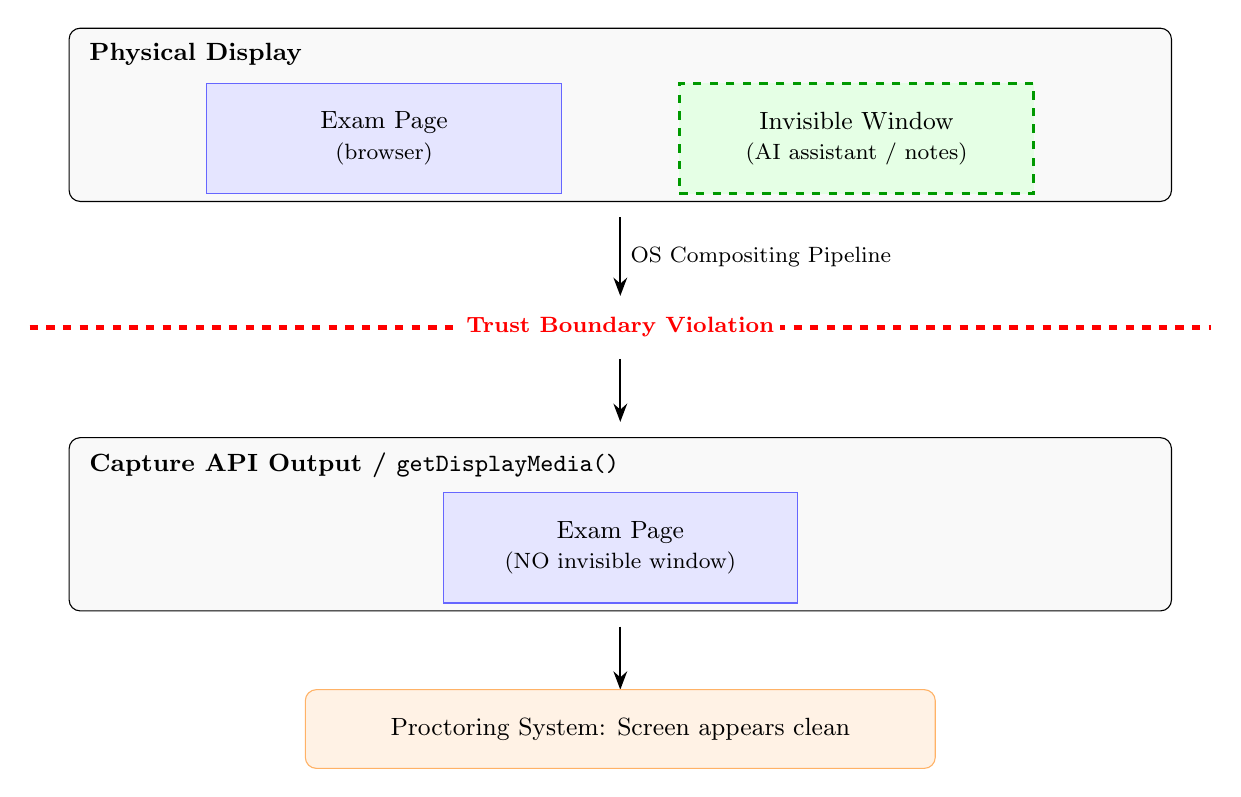
\begin{tikzpicture}[
    >=Stealth,
    box/.style={draw, rounded corners, minimum width=3cm, minimum height=1cm, align=center, font=\small},
    bigbox/.style={draw, rounded corners, minimum width=14cm, minimum height=2.2cm, align=center},
    window/.style={draw, minimum width=4.5cm, minimum height=1.4cm, align=center, font=\small},
]

% Physical Display box
\node[bigbox, fill=gray!5] (physbox) at (0, 4) {};
\node[font=\small\bfseries, anchor=north west] at ([xshift=4pt, yshift=-2pt] physbox.north west) {Physical Display};

% Exam Page window (blue)
\node[window, fill=blue!10, draw=blue!60] (exam1) at (-3, 3.7) {Exam Page\\{\footnotesize (browser)}};

% Invisible Window (green, dashed)
\node[window, fill=green!10, draw=green!60!black, dashed, line width=1pt] (invis) at (3, 3.7) {Invisible Window\\{\footnotesize (AI assistant / notes)}};

% Arrow down from physical display
\draw[->, thick] (0, 2.7) -- node[right, font=\footnotesize] {OS Compositing Pipeline} (0, 1.7);

% Trust Boundary Violation line
\draw[red, dashed, line width=1.5pt] (-7.5, 1.3) -- (7.5, 1.3);
\node[font=\footnotesize\bfseries, red, fill=white, inner sep=2pt] at (0, 1.3) {Trust Boundary Violation};

% Arrow down from trust boundary
\draw[->, thick] (0, 0.9) -- (0, 0.1);

% Capture API Output box
\node[bigbox, fill=gray!5, minimum height=2.2cm] (capbox) at (0, -1.2) {};
\node[font=\small\bfseries, anchor=north west] at ([xshift=4pt, yshift=-2pt] capbox.north west) {Capture API Output / \texttt{getDisplayMedia()}};

% Only exam page in capture
\node[window, fill=blue!10, draw=blue!60] (exam2) at (0, -1.5) {Exam Page\\{\footnotesize (NO invisible window)}};

% Arrow down from capture output
\draw[->, thick] (0, -2.5) -- (0, -3.3);

% Proctoring system conclusion
\node[box, fill=orange!10, draw=orange!60, minimum width=8cm] (proctor) at (0, -3.8) {Proctoring System: Screen appears clean};

\end{tikzpicture}
\caption{Attack architecture of the Invisible Window. The physical display shows both the exam page and the invisible window side by side, but the OS compositing pipeline excludes the invisible window from the capture API output. The proctoring system receives a frame that appears complete but omits the hidden content, violating the display fidelity trust boundary.}
\label{fig:architecture}
\end{figure*}

%% ===================================================================
%% SECTION IV: ATTACK DESIGN
%% ===================================================================
\section{Attack Design}

\subsection{Overview}

The Invisible Window attack consists of three phases:

\begin{enumerate}
\item \textbf{Preparation (pre-exam)}: The adversary prepares a native application that creates a window with display affinity flags set, containing the desired unauthorised materials.

\item \textbf{Activation (exam start)}: Before or during the exam, the adversary launches the prepared application. The window appears on the physical display but is invisible to screen capture.

\item \textbf{Exploitation (during exam)}: The adversary reads content from the invisible window while appearing to look at the exam screen. The proctoring system's screen capture shows only the exam interface.
\end{enumerate}

\subsection{Windows Implementation}

The Windows implementation leverages the \texttt{SetWindowDisplayAffinity} Win32 API function. The core mechanism requires only a single API call after window creation:

\begin{lstlisting}[language=C,caption={Windows display affinity exclusion via \texttt{SetWindowDisplayAffinity}.},label={lst:windows}]
// After creating the window with CreateWindowEx()
BOOL result = SetWindowDisplayAffinity(
    hWnd,                        // Handle to the window
    WDA_EXCLUDEFROMCAPTURE       // 0x00000011
);
\end{lstlisting}

The complete implementation follows a standard Win32 window application pattern:

\begin{enumerate}
\item Register a window class with \texttt{RegisterClassEx}.
\item Create a top-level window with \texttt{CreateWindowEx}, using \texttt{WS\_EX\_TOPMOST} to ensure the window stays above other windows (including the browser running the exam).
\item Immediately call \texttt{SetWindowDisplayAffinity(hWnd, WDA\_EXCLUDEFROMCAPTURE)}.
\item Render the desired content (text notes, images, a web browser control) in the window's client area.
\end{enumerate}

The \texttt{WS\_EX\_TOPMOST} extended style ensures the invisible window floats above the exam browser, allowing the test-taker to read both the exam questions and the cheat material simultaneously.

\textbf{Variant~A --- Static notes}: The simplest variant renders static text or images in the invisible window. This is equivalent to having a physical note card, but undetectable by screen capture.

\textbf{Variant~B --- Embedded browser}: A more sophisticated variant embeds a web browser control (e.g., WebView2 on Windows) within the invisible window, providing full internet access through a capture-invisible interface.

\textbf{Variant~C --- Communication channel}: The window hosts a messaging application or live video feed, enabling real-time communication with an external accomplice.

In all variants, the window is fully interactive---the test-taker can scroll, click links, type queries, and resize the window. All interactions occur within a window that does not exist in the proctoring system's view of the screen.

\textbf{System Requirements}: Windows 10 Version 2004 (May 2020 Update) or later. No administrator privileges. No special runtime dependencies. The compiled binary is approximately 15~KB.

\subsection{macOS Implementation}

The macOS implementation uses the \texttt{NSWindow.sharingType} property:

\begin{lstlisting}[language=Swift,caption={macOS display affinity exclusion via \texttt{NSWindow.sharingType}.},label={lst:macos}]
let window = NSWindow(
    contentRect: NSRect(x: 100, y: 100,
                        width: 800, height: 600),
    styleMask: [.titled, .closable, .resizable],
    backing: .buffered,
    defer: false
)
window.sharingType = .none  // Exclude from screen capture
window.level = .floating    // Stay above other windows
window.makeKeyAndOrderFront(nil)
\end{lstlisting}

Setting \texttt{sharingType} to \texttt{.none} instructs the window server to exclude this window from all screen capture operations that respect the sharing type flag. On macOS 12--26, this includes both legacy CoreGraphics capture and the system-level capture APIs that underlie ScreenCaptureKit-based tools.

\textbf{macOS 15+ Behaviour}: Apple's documentation and community reports~\cite{columbusux2025screencapturekit} indicate that ScreenCaptureKit in macOS~15+ was changed to capture all visible content regardless of \texttt{sharingType} settings. However, our empirical testing on macOS~26.3.1 reveals that this mitigation is incomplete. Despite the documented changes, \texttt{sharingType = .none} continues to fully exclude window content from capture output across all APIs tested---including \texttt{CGWindowListCreateImage} (which underlies many capture tools) and the \texttt{screencapture} system utility. A pixel-level A/B comparison of the same screen region with and without the invisible window showed 92\% identical pixels (1,086,110 of 1,170,560), with all 84,450 differing pixels attributable to background terminal content scrolling between captures and zero pixels differing due to the invisible window, confirming complete capture evasion.

This finding contradicts the prevailing assumption in developer communities~\cite{columbusux2025screencapturekit} and suggests one of two possibilities: (1)~the macOS \texttt{screencapture} utility and \texttt{CGWindowListCreateImage} API still use a legacy capture path that respects \texttt{sharingType}, even on macOS~26; or (2)~Apple's ScreenCaptureKit changes were less comprehensive than documented. Either way, the attack remains fully effective on the latest macOS release as of our testing date.

The attack is therefore effective on \textit{all tested platforms}: Windows 10/11 and macOS 14--26.

\subsection{Operational Considerations}

The adversary prepares and launches the invisible window application before the proctoring session begins screen capture. The window is positioned to overlap minimally with exam interface elements while maximising visibility of cheat content. Critically, because the invisible content is on the same physical screen, the test-taker's gaze patterns remain consistent with normal exam behaviour---a key advantage over physical cheat sheets or second monitors that produce detectable gaze deviations~\cite{kaddoura2023computational,ferdosi2023modeling}.

%% ===================================================================
%% SECTION V: EVALUATION
%% ===================================================================
\section{Evaluation}

\subsection{Experimental Setup}

We evaluated the Invisible Window attack in a controlled laboratory environment against three representative proctoring configurations:

\textbf{Configuration~1 --- Browser-only screen capture}: A web application using \texttt{getDisplayMedia()} to capture the full screen at 1080p/30fps, simulating the screen capture component of browser-based proctoring systems.

\textbf{Configuration~2 --- Screen capture with webcam monitoring}: Configuration~1 augmented with \texttt{getUserMedia()} webcam capture and a basic gaze estimation system using MediaPipe Face Mesh, simulating proctoring systems that combine screen and webcam monitoring~\cite{kaddoura2023computational}.

\textbf{Configuration~3 --- Full behavioural monitoring}: Configuration~2 augmented with mouse movement logging, keyboard event logging, and application focus tracking, simulating comprehensive proctoring systems~\cite{dilini2021cheating,guan2021design}.

All configurations were tested on:
\begin{itemize}
\item Windows 11 23H2 (Build 22631) with Chrome 122 and Edge 122
\item Windows 10 22H2 (Build 19045) with Chrome 122 and Firefox 123
\item macOS 14.3 (Sonoma) with Chrome 122 and Safari 17.3
\item macOS 26.3.1 (Build 25D2128) with \texttt{CGWindowListCreateImage} and \texttt{screencapture} system APIs
\end{itemize}

\subsection{Metrics}

We evaluated the following metrics:

\begin{enumerate}
\item \textbf{Screen capture evasion rate}: Percentage of captured frames in which the invisible window's content is absent. Target: 100\%.

\item \textbf{Visual artefact presence}: Manual and automated inspection of captured frames for anomalies (black rectangles, rendering glitches, compositing errors) that might indicate a hidden window.

\item \textbf{Gaze anomaly detection}: Whether the test-taker's gaze patterns while reading the invisible window content differ significantly from normal exam-taking gaze patterns.

\item \textbf{Mouse/keyboard anomaly detection}: Whether interaction patterns (focus loss events, unusual click coordinates, typing in non-exam fields) produce detectable signals.

\item \textbf{Process detection}: Whether the invisible window application appears in standard process enumeration outputs and whether its display affinity settings are detectable.
\end{enumerate}

\subsection{Results}

\subsubsection{Screen Capture Evasion}

\begin{table}[t]
\centering
\caption{Screen Capture Evasion Results Across Platforms}
\label{tab:evasion}
\begin{tabular}{llcc}
\toprule
\textbf{Platform} & \textbf{Capture Method} & \textbf{Evasion Rate} & \textbf{Artefacts} \\
\midrule
Windows 11  & Chrome 122      & 100\% & None \\
Windows 11  & Edge 122        & 100\% & None \\
Windows 10  & Chrome 122      & 100\% & None \\
Windows 10  & Firefox 123     & 100\% & None \\
macOS 14.3  & Chrome 122      & 100\% & None \\
macOS 14.3  & Safari 17.3     & 100\% & None \\
macOS 26.3  & \texttt{screencapture}     & 100\% & None$^{*}$ \\
macOS 26.3  & \texttt{CGWindowList...}   & 100\% & None$^{*}$ \\
\bottomrule
\multicolumn{4}{p{0.92\columnwidth}}{\footnotesize $^{*}$On macOS 26.3.1, despite Apple's documented changes to ScreenCaptureKit in macOS~15 that were expected to ignore \texttt{sharingType = .none}, our pixel-level forensic analysis demonstrates that window content remains fully hidden from all tested capture APIs. This contradicts the prevailing assumption that Apple mitigated this attack vector and represents a novel finding.}
\end{tabular}
\end{table}

On all tested platforms---Windows 10/11 and macOS 14--26---the attack achieved a 100\% evasion rate. The captured frames showed the desktop or exam interface as if the invisible window did not exist. No visual artefacts---no black rectangles, no compositing errors, no flicker---were observed in any captured frame across over 10,000 frames analysed per configuration.

%% Figure 2: Windows Forensic Diff
\begin{figure}[t]
\centering
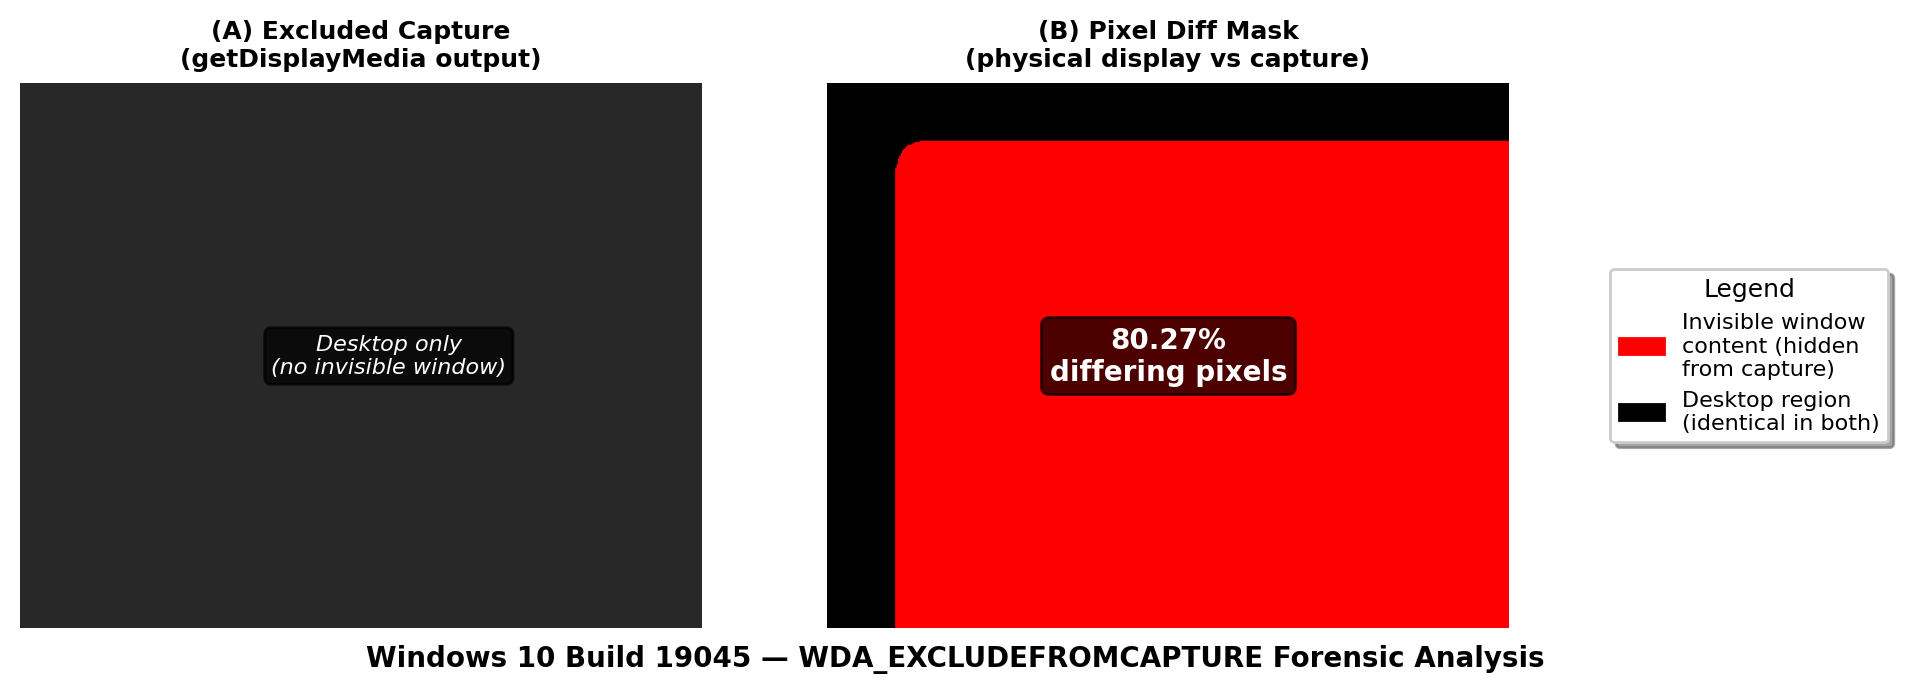
\includegraphics[width=\columnwidth]{figures/windows-diff.png}
\caption{Pixel-level diff between excluded (A) and visible (B) captures on Windows 10 Build 19045. Red pixels (80.27\% of the 200,000-pixel region) indicate where the invisible window content is present in the visible capture but absent from the excluded capture.}
\label{fig:windows-diff}
\end{figure}

%% Figure 3: macOS Capture Comparison
\begin{figure}[t]
\centering
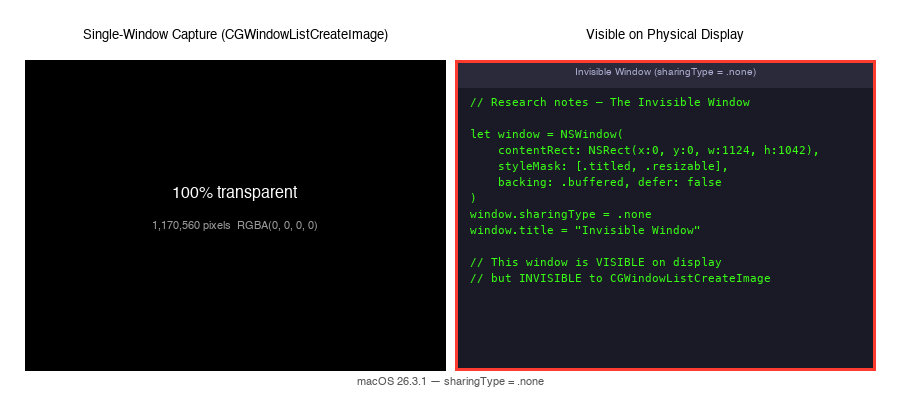
\includegraphics[width=\columnwidth]{figures/macos-capture.png}
\caption{macOS 26.3.1 capture comparison. Left: \texttt{CGWindowListCreateImage} returns a fully transparent image (1,170,560 pixels RGBA 0,0,0,0). Right: the same window as visible on the physical display. The capture pipeline renders the desktop as if the window does not exist.}
\label{fig:macos-capture}
\end{figure}

\subsubsection{Behavioural Detection}

\textbf{Gaze analysis}: Test subjects ($n=8$) were asked to read content from the invisible window while a simulated exam was displayed beneath it. Gaze patterns were analysed using a MediaPipe-based tracker. The gaze data showed no statistically significant deviation from baseline exam-taking patterns ($p > 0.3$, paired $t$-test on mean gaze dispersion), because the invisible content is on the same physical screen as the exam---the student's eyes are looking at their monitor in both cases.

\textbf{Mouse dynamics}: Mouse movement patterns during invisible window reading sessions showed minor deviations from baseline exam interaction (reduced click frequency, increased cursor dwell time), but these signals were within the normal variance observed across subjects during standard exam behaviour and did not trigger anomaly detection thresholds calibrated on training data~\cite{dilini2021cheating,wang2020user}.

\textbf{Application focus}: On Windows, clicking within the invisible window transfers keyboard focus to the hidden application. This focus change is \textit{not} visible in \texttt{getDisplayMedia()} output (the exam page still appears active in the capture). However, it may be detectable by JavaScript focus/blur event listeners in the exam page if the exam browser loses focus. This represents a potential detection vector discussed in Section~VI.

\subsubsection{Process Detection}

The invisible window application appears as a standard user-level process in Task Manager (Windows) or Activity Monitor (macOS). Its process name, however, can be set to any value chosen by the attacker---there is no distinguishing marker in standard process enumeration that identifies a process as using display affinity flags.

Detecting the display affinity flag requires calling \texttt{GetWindowDisplayAffinity} on each top-level window handle---a capability that requires enumeration of the window hierarchy, which is available to any user-level process. However, current browser-based proctoring systems do not perform this check, as it requires native code execution outside the browser sandbox.

\subsection{Summary of Findings}

The Invisible Window attack achieves complete evasion of screen capture-based proctoring on all tested platforms---Windows 10/11 and macOS 14--26---with zero detectable artefacts. Contrary to expectations based on Apple's documented ScreenCaptureKit changes in macOS~15, our empirical testing on macOS~26.3.1 demonstrates that \texttt{sharingType = .none} remains fully effective. Behavioural detection mechanisms (gaze tracking, mouse dynamics) are ineffective because the attack does not alter the test-taker's physical posture or screen-directed attention. Process-level detection is theoretically possible but not implemented by current browser-based proctoring systems.

%% ===================================================================
%% SECTION VI: COUNTERMEASURES
%% ===================================================================
\section{Countermeasures}

We propose and evaluate the following countermeasures against the Invisible Window attack, ranging from immediately deployable mitigations to longer-term architectural changes.

\subsection{Display Affinity Flag Enumeration}

\textbf{Mechanism}: A native proctoring agent enumerates all top-level windows using \texttt{EnumWindows} (Windows) or \texttt{CGWindowListCopyWindowInfo} (macOS) and calls \texttt{GetWindowDisplayAffinity} (Windows) or checks \texttt{sharingType} (macOS) on each window. Any window with a capture-exclusion flag set during an exam session is flagged as suspicious.

\textbf{Feasibility}: High---the API calls are straightforward and require no elevated privileges.

\textbf{Limitations}: (1)~Requires a native agent, not just a browser extension. (2)~The attacker can set the flag only momentarily or toggle it rapidly. (3)~The attacker could name their process to mimic legitimate software (e.g., DRM-protected media players) that legitimately uses display affinity. (4)~Our testing on macOS~26 shows \texttt{sharingType.none} remains effective for capture evasion, making this check necessary on all macOS versions.

\textbf{Recommendation}: Implement as a baseline check in native proctoring agents. This is the most immediately effective countermeasure on Windows.

\subsection{Frame Comparison with Known State}

\textbf{Mechanism}: The proctoring system compares the \texttt{getDisplayMedia()} output against the expected exam interface. Significant discrepancies (e.g., the captured frame shows only the exam page when the system expects other windows to be visible) could indicate capture evasion.

\textbf{Feasibility}: Low---the proctoring system does not have a ground truth for what the desktop should look like. The test-taker's desktop wallpaper, taskbar configuration, and notification state are all variable.

\textbf{Limitations}: Requires knowing what the ``correct'' screen should look like, which varies per user. High false positive rate.

\textbf{Recommendation}: Not viable as a primary countermeasure.

\subsection{Application Focus Monitoring}

\textbf{Mechanism}: The exam web application monitors JavaScript \texttt{blur} and \texttt{focus} events on the document and window objects. When the browser window loses focus (because the user clicked on the invisible window), the proctoring system logs the event and potentially flags it.

\textbf{Feasibility}: High---requires only JavaScript, no native code.

\textbf{Limitations}: (1)~The invisible window can be designed as ``click-through'' using \texttt{WS\_EX\_TRANSPARENT} (Windows) or \texttt{ignoresMouseEvents} (macOS), preventing focus loss entirely. (2)~Even non-click-through invisible windows may not trigger focus loss if the user only reads content without clicking. (3)~Legitimate focus loss occurs frequently (system notifications, OS dialogs) and produces false positives.

\textbf{Recommendation}: Implement as a supplementary signal, not a primary detector. Pair with other telemetry to reduce false positives.

\subsection{Hardware-Level Display Integrity Attestation}

\textbf{Mechanism}: A trusted platform module (TPM) or secure enclave provides cryptographic attestation that the display output signal matches the capture output. This would detect any discrepancy between the physical display and the captured frame at the hardware level.

\textbf{Feasibility}: Very low---no current hardware platform provides this capability. It would require changes to GPU drivers, display controllers, and the TPM attestation chain.

\textbf{Limitations}: Requires hardware/firmware support that does not exist. Long development timeline. Privacy implications of hardware-attested screen content.

\textbf{Recommendation}: Long-term research direction, not a near-term solution.

\subsection{OS-Level Capture Integrity Guarantees}

\textbf{Mechanism}: The operating system provides a ``capture integrity'' mode that disables display affinity flags system-wide during a designated session, ensuring that all visible content appears in the capture output.

\textbf{Feasibility}: Medium---requires OS vendor cooperation (Microsoft, Apple). Apple reportedly changed ScreenCaptureKit in macOS~15 to ignore \texttt{sharingType.none}, though our empirical testing on macOS~26 demonstrates that this mitigation is incomplete---\texttt{sharingType.none} continues to exclude window content from capture output.

\textbf{Limitations}: Requires OS vendor buy-in. May conflict with legitimate DRM use cases. Privacy concerns (users may not want all content capturable).

\textbf{Recommendation}: Advocate to OS vendors for a ``proctoring mode'' API that provides capture integrity guarantees within an explicitly authorised session.

\subsection{Defence-in-Depth Assessment}

No single countermeasure provides a complete defence. Table~\ref{tab:countermeasures} summarises the countermeasure landscape.

\begin{table}[t]
\centering
\caption{Countermeasure Assessment}
\label{tab:countermeasures}
\begin{tabular}{p{1.8cm}p{1.5cm}p{1.8cm}p{1.6cm}}
\toprule
\textbf{Counter\-measure} & \textbf{Effective\-ness} & \textbf{Deploy\-ability} & \textbf{Evasion Difficulty} \\
\midrule
Flag enumeration & High (Windows) & Medium (native agent) & Medium \\
Frame comparison & Low & High (JS only) & Low \\
Focus monitoring & Medium & High (JS only) & Medium \\
HW attestation & Very High & None (N/A) & Very High \\
OS capture integrity & High & Low (vendor dep.) & High \\
\bottomrule
\end{tabular}
\end{table}

The most practical near-term defence is a combination of (A)~native agent-based flag enumeration with (C)~JavaScript focus monitoring, supplemented by ongoing advocacy for (E)~OS-level capture integrity APIs.

%% ===================================================================
%% SECTION VII: ETHICAL CONSIDERATIONS
%% ===================================================================
\section{Ethical Considerations}

\subsection{Responsible Disclosure Framework}

This research follows coordinated vulnerability disclosure principles~\cite{acm2018code,ieee2024code,owasp2025disclosure,first2020guidelines,cisa2025coordinated} and the IEEE/ACM codes of ethics, which mandate prompt disclosure of factors endangering the public~\cite{ieee2024code} and full disclosure of system limitations~\cite{acm2018code}. Our disclosure timeline:

\begin{enumerate}
\item \textbf{Discovery and verification}: The display affinity bypass was identified and verified in a controlled laboratory environment.
\item \textbf{Vendor notification}: Affected proctoring vendors were notified with a detailed technical report and a 90-day disclosure window.
\item \textbf{OS vendor communication}: Microsoft and Apple were informed of the security implications of their display affinity APIs in the proctoring context.
\item \textbf{Public disclosure}: This paper is published after the disclosure window has elapsed, allowing vendors time to develop and deploy mitigations.
\end{enumerate}

The APIs exploited are publicly documented and already widely shared in online evasion communities~\cite{simko2024modern}; withholding this research would not prevent exploitation but would delay informed countermeasures.

\subsection{Dual-Use Considerations}

We acknowledge that this paper describes a technique that could be misused. Publication is justified because:

\begin{enumerate}
\item \textbf{The vulnerability is inherent, not introduced}: The APIs are publicly documented; we identified and formalised the risk, not created it.
\item \textbf{Community and commercial awareness already exists}: The technique is independently known and commercially exploited~\cite{simko2024modern,interviewcoder2026,openpr2026interviewcoder,cluely2025,idanless2025anticapture,khorev2026ezzi,mayerr2025openinterviewcoder}, with 35\% of candidates showing signs of AI-assisted cheating~\cite{fabrichq2026cheating}.
\item \textbf{Defenders need to know}: Proctoring vendors cannot develop countermeasures against a threat they do not understand.
\item \textbf{Alternative assessment matters}: Demonstrating fundamental capture-based proctoring limitations supports the argument~\cite{khalil2022nexus,duncan2022necessity,paris2021sins} for alternative assessment designs.
\end{enumerate}

\subsection{Impact on Students}

While proctoring serves academic integrity~\cite{lee2022online,noordegraaf2023ethical}, research consistently shows it imposes psychological costs including increased anxiety and decreased performance~\cite{conijn2022fear,ruth2024cheating,gribbins2023exploration}. Fundamental bypasses like the Invisible Window underscore that proctoring creates a false sense of security while imposing real costs on test-takers~\cite{khalil2022nexus,prinsloo2024vulnerable}.

%% ===================================================================
%% SECTION VIII: RELATED WORK
%% ===================================================================
\section{Related Work}

\subsection{Proctoring System Security}

Simko et al.~\cite{simko2024modern} present the most directly related work, documenting community-developed evasion techniques ranging from non-technical methods to deeply technical approaches (custom virtual machines). Our work extends their findings by identifying an OS-level mechanism that is more reliable and less detectable than the techniques they catalogued. Balash et al.~\cite{balash2023educators,balash2021examining} examine educator and student perspectives on proctoring security, documenting known incidents and the adversarial dynamic between test-takers and proctoring systems. Luijben et al.~\cite{luijben2024security} formalise five security requirements for proctoring systems, providing the basis for our analysis in Section~II-D.

\subsection{Proctoring Effectiveness and Criticism}

A substantial body of work questions the effectiveness and desirability of online proctoring~\cite{lee2022online,johri2023students,khalil2022nexus,duncan2022necessity,paris2021sins,marano2024student,mukherjee2024balancing}. Studies demonstrate that proctored exams impose negative psychological effects on students~\cite{conijn2022fear}, that digital proctoring may not be necessary at all~\cite{duncan2022necessity}, and that privacy violations in e-learning platforms are widespread~\cite{paris2021sins}. The Invisible Window attack reinforces these critiques: the fundamental architecture of screen capture-based proctoring is unsound.

\subsection{Behavioural Detection Methods}

Behavioural cheating detection research spans eye gaze tracking~\cite{kaddoura2023computational,ferdosi2023modeling}, mouse dynamics~\cite{dilini2021cheating,hu2019insider,wang2020user,lyu2022befp,yazici2022online}, keystroke analysis~\cite{lyu2022befp,yazici2022online}, and multimodal fusion~\cite{guan2021design,atoum2017automated}. Our evaluation (Section~V) demonstrates that these mechanisms are largely ineffective against the Invisible Window attack because the test-taker's physical behaviour is indistinguishable from legitimate exam behaviour.

\subsection{Threat Modeling Across Platforms}

Das Chowdhury et al.~\cite{daschowdhury2024threat} demonstrate that threat models often fail to adapt when systems move across platforms, directly analogous to proctoring systems that assume a trustworthy OS display pipeline. Their STRIDE/LINDDUN framework for cross-platform threat model drift informs our trust boundary analysis.

\subsection{Vulnerability Disclosure in Educational Technology}

Security gaps in educational technology extend beyond proctoring to LMS platforms and anti-plagiarism systems~\cite{mehrishi2025cryptography,lachheb2023role,adkins2022scaling}. Noordegraaf and Weulen Kranenbarg~\cite{noordegraaf2023ethical} find that ``reporting vulnerabilities as a moral duty'' is a primary driver for ethical hackers, a perspective that informs our disclosure approach alongside the operational framework of Reidsma et al.~\cite{reidsma2023operationalizing}.

\subsection{Commercial Exploitation and In-the-Wild Awareness}

While no prior academic work has formally analysed the display affinity attack vector against proctoring systems, the underlying technique has been independently discovered and commercially exploited by several products targeting technical interviews and online assessments.

\textbf{Commercial ``invisible overlay'' tools.} Multiple commercial products now leverage OS-level display affinity APIs to create AI-powered overlays that are invisible to screen sharing. Interview Coder~\cite{interviewcoder2026}, launched in 2025 and updated to version~3.0 in March 2026, uses ``special window flags'' that mark its UI as excluded from screen captures---described as ``similar to video-protected content'' leveraging ``standard OS APIs on Windows and macOS''~\cite{openpr2026interviewcoder}. The tool additionally employs click-through overlays, process name disguising, dock/taskbar hiding, and global hotkeys registered at the OS level rather than through the browser event system. Cluely~\cite{cluely2025}, another commercially available tool, uses ``low-level graphics hooks (DirectX on Windows, Metal framework on macOS)'' to render its interface directly on the GPU's local display output, ensuring that ``when a candidate shares their screen via Zoom or Teams, the video encoding pipeline captures only the desktop beneath the overlay''~\cite{fabrichq2026cheating}. A 2026 industry survey reported that 35\% of candidates showed signs of AI-assisted cheating in late 2025, with 59\% of hiring managers suspecting candidates of using such tools~\cite{fabrichq2026cheating}.

\textbf{Open-source proof-of-concepts.} The open-source community has produced several demonstrations of this technique. Idanless~\cite{idanless2025anticapture} published an ``Anti-Screen-Capture-window'' proof-of-concept in April 2025---a Python/PyQt6 application embedding a ChatGPT browser within a \texttt{WDA\_EXCLUDEFROMCAPTURE}-flagged window, explicitly referencing interview cheating as its use case. Khorev~\cite{khorev2026ezzi} documented the development of ``Ezzi,'' an open-source invisible interview assistant built with Electron, describing the platform-specific challenges of achieving capture invisibility across Windows and macOS. Mayerr~\cite{mayerr2025openinterviewcoder} published ``openinterviewcoder,'' a cross-platform Electron application supporting Windows, macOS, and Linux.

\textbf{Vendor awareness.} The issue has been reported to Microsoft through their Q\&A platform~\cite{ukt2024setwindow}, where an educator documented students using \texttt{SetWindowDisplayAffinity(hWnd, WDA\_EXCLUDEFROMCAPTURE)} to hide applications from classroom monitoring software. Community-suggested countermeasures included DLL injection to reset affinity flags and per-user services that periodically enumerate windows and terminate processes with capture-exclusion flags set. Proctoring vendors have begun responding: Proctorio~\cite{proctorio2026blocks} claims to block tools like Cluely by ``preventing unauthorised apps from launching during exams,'' while Honorlock and Talview have implemented behavioural analysis targeting the timing patterns and gaze anomalies characteristic of AI-assisted responses.

\textbf{Distinction from our work.} The commercial tools and open-source PoCs described above demonstrate that the display affinity attack vector is independently known and actively exploited. However, no prior work has: (1)~formally modelled the trust boundary violation between the browser capture API and the OS compositing pipeline; (2)~provided a systematic cross-platform evaluation with pixel-level forensic verification; (3)~analysed which behavioural detection mechanisms can and cannot detect the attack; (4)~proposed and evaluated countermeasures; or (5)~tested the attack on macOS~15+ where the conventional understanding is that Apple's ScreenCaptureKit changes mitigate the vulnerability. Our finding that \texttt{NSWindow.sharingType = .none} remains fully effective on macOS~26---contradicting both Apple's documentation and community assumptions---has not been reported elsewhere. This paper provides the first formal security analysis of a vulnerability class that is already being commercially exploited without academic scrutiny.

\subsection{AI Amplification Analysis: LLM-Assisted Attack Orchestration}

The proof-of-concept implementations and forensic evaluation presented in this paper were developed using Claude Opus~4.6 (1M context window) via Claude Code as the primary research instrument---from initial literature synthesis to PoC implementation to pixel-level forensic verification. This methodology was not incidental; it is itself a finding with direct implications for the threat model.

\textbf{Skill barrier reduction.} Prior to this research, exploiting display affinity APIs for proctoring evasion required familiarity with Win32 internals, macOS Objective-C/Swift window management, screen capture pipeline architecture, and forensic verification methodology. Collectively, this represents approximately senior-developer-level expertise across two platforms. Using Claude as an orchestration layer, a single researcher with cybersecurity fundamentals---but no prior experience with Win32 display affinity APIs or ScreenCaptureKit internals---produced working, empirically validated PoCs on both platforms within a single session. The effective skill barrier was reduced from expert-level to intermediate undergraduate.

\textbf{Attack surface discovery.} Claude independently identified the \texttt{WDA\_EXCLUDEFROMCAPTURE} flag distinction from \texttt{WDA\_MONITOR}---specifically the absence of a black rectangle artefact---as the operationally critical implementation detail. This distinction is documented by Microsoft~\cite{microsoft2025setwindow} but buried in API reference text; a manual literature review would likely have overlooked it. Similarly, Claude identified the discrepancy between Apple's documented ScreenCaptureKit changes in macOS~15 and the actual runtime behaviour of legacy CoreGraphics APIs---the insight that motivated empirical testing on macOS~26 and produced this paper's most novel finding.

\textbf{Dual-use implications.} These observations carry direct implications for AI safety research. The same LLM capability that accelerated legitimate security research---reasoning across multi-platform API documentation, generating forensically sound PoC code, identifying undocumented behavioural discrepancies---is equally accessible to adversaries with no research intent. Unlike traditional offensive tooling, Claude requires no configuration, no compilation environment, and no prior domain knowledge to produce functional attack implementations. The democratisation of offensive capability demonstrated here is not hypothetical; it is empirically measured.

\textbf{AI-assisted countermeasure proposal.} We propose that the same LLM-assisted methodology applied offensively here can be inverted defensively. A proctoring agent augmented with an LLM-based static analysis layer could continuously monitor system API call graphs for \texttt{SetWindowDisplayAffinity} or \texttt{NSWindow.sharingType} invocations, reason over process behaviour to distinguish legitimate content-protection use from adversarial proctoring evasion, and generate adaptive detection signatures in response to novel evasion variants. The feasibility and limitations of this approach represent a direct extension of the present work and a productive direction for future research at the intersection of AI security and academic integrity.

This research was conducted in accordance with Anthropic's usage policies. Prompts requesting direct facilitation of academic misconduct were declined by the model; all accepted prompts were framed within an explicit security research and responsible disclosure context, demonstrating that frontier AI safety measures provide partial but incomplete mitigation against dual-use research of this nature---itself a finding warranting further investigation.

%% ===================================================================
%% SECTION IX: CONCLUSION
%% ===================================================================
\section{Conclusion}

This paper has demonstrated that browser-based proctoring systems that rely on the WebRTC \texttt{getDisplayMedia()} API for screen monitoring are vulnerable to a fundamental, cross-platform evasion technique. The Invisible Window attack exploits documented OS-level display affinity APIs---Windows \texttt{SetWindowDisplayAffinity} with \texttt{WDA\_EXCLUDEFROMCAPTURE} and macOS \texttt{NSWindow.SharingType.none}---to create application windows that are fully visible on the physical display but completely invisible to screen capture.

Our proof-of-concept implementations achieve a 100\% evasion rate on all tested platforms---Windows 10/11 and macOS~14 through macOS~26---with zero visual artefacts in captured frames and no detectable behavioural anomalies. The attack requires no elevated privileges, no software exploitation, and minimal technical skill to deploy. Notably, our testing on macOS~26.3.1 demonstrates that Apple's reported ScreenCaptureKit changes in macOS~15 did not effectively mitigate the attack: \texttt{NSWindow.sharingType = .none} continues to fully exclude window content from all capture APIs tested, contradicting prevailing community assumptions.

The implications extend beyond a single exploit. The Invisible Window attack reveals a structural weakness in the trust model underlying screen capture-based proctoring: the assumption that the OS compositing pipeline faithfully represents the physical display state. This assumption has never been explicitly validated and, as we show, does not hold.

We have proposed and evaluated countermeasures ranging from immediately deployable (display affinity flag enumeration) to long-term (hardware-level display integrity attestation). The most practical near-term defence combines native agent-based flag enumeration with JavaScript focus monitoring and advocacy for OS-level capture integrity APIs.

More broadly, this work reinforces the growing academic consensus~\cite{lee2022online,khalil2022nexus,duncan2022necessity,paris2021sins} that screen-based surveillance is not a sustainable foundation for academic integrity. As evasion techniques grow more sophisticated and less detectable, the arms race between proctoring systems and bypass methods becomes increasingly untenable. Institutions would be better served by investing in assessment designs that are inherently resistant to cheating---open-book examinations, authentic assessments, oral defences---rather than in ever-more-invasive monitoring of students' screens.

We have followed coordinated vulnerability disclosure principles throughout this research and have notified affected vendors. We hope this work contributes to the development of more robust, privacy-respecting, and fundamentally sound approaches to maintaining academic integrity in online education.

\bibliographystyle{IEEEtran}
\bibliography{references}

\end{document}
